\documentclass{article}
\pdfoutput=1 

% if you need to pass options to natbib, use, e.g.:
    \PassOptionsToPackage{numbers, compress}{natbib}
% before loading neurips_2022


% ready for submission
% \usepackage{neurips_2022}


% to compile a preprint version, e.g., for submission to arXiv, add add the
% [preprint] option:
    % \usepackage[preprint]{neurips_2022}


% to compile a camera-ready version, add the [final] option, e.g.:
\usepackage[final]{neurips2022}


% to avoid loading the natbib package, add option nonatbib:
% \usepackage[nonatbib]{neurips_2022}


\usepackage[utf8]{inputenc} % allow utf-8 input
\usepackage[T1]{fontenc}    % use 8-bit T1 fonts
\usepackage{hyperref}       % hyperlinks
\usepackage{url}            % simple URL typesetting
\usepackage{booktabs}       % professional-quality tables
\usepackage{amsfonts}       % blackboard math symbols
\usepackage{nicefrac}       % compact symbols for 1/2, etc.
\usepackage{microtype}      % microtypography
\usepackage{xcolor}         % colors

\usepackage{amsmath,amsthm,amssymb,amsfonts,amscd,keyval}
\usepackage{bm}
\usepackage{mathtools}
\usepackage{multirow}
\usepackage{dsfont}
\usepackage{float}
\usepackage{xspace}
\usepackage{subfig}
\usepackage{bbding}
\usepackage{makecell}


\newcommand{\methodfull}{\textsc{Brain Network Transformer}\xspace}
% \newcommand{\methodshort}{\textsc{BrainTransformer}\xspace}
\newcommand{\methodtable}{\textsc{BrainNetTF}\xspace}
\newcommand{\pooling}{\textsc{Orthonormal Clustering Readout}\xspace}
\newcommand{\poolingshort}{\textsc{OCRead}\xspace}
\newcommand{\ie}{\textit{i.e.}}
\newcommand{\eg}{\textit{e.g.}}
\newcommand{\xkan}[1]{{\color{blue}{#1}}}
\newcommand{\dvd}[1]{{\color{red}{#1}}}
\newcommand{\hejie}[1]{{\color{blue}{#1}}}
\newcommand{\zzl}[1]{{\color{brown}{#1}}}

\theoremstyle{definition}
\newtheorem{definition}{Definition}[section]
\newtheorem*{example}{Example}
\newtheorem{proposition}[definition]{Proposition}

\theoremstyle{plain}
\newtheorem{theorem}[definition]{Theorem}
\newtheorem{lemma}[definition]{Lemma}
\newtheorem{corollary}[definition]{Corollary}

\theoremstyle{remark}
\newtheorem*{remark}{Remark}

\title{\methodfull}


% The \author macro works with any number of authors. There are two commands
% used to separate the names and addresses of multiple authors: \And and \AND.
%
% Using \And between authors leaves it to LaTeX to determine where to break the
% lines. Using \AND forces a line break at that point. So, if LaTeX puts 3 of 4
% authors names on the first line, and the last on the second line, try using
% \AND instead of \And before the third author name.


\author{%
Xuan Kan$^1$ \quad Wei Dai$^2$ \quad Hejie Cui$^1$ \quad Zilong Zhang$^3$ \quad Ying Guo$^1$ \quad Carl Yang$^1$\\
$^1$Emory University \quad $^2$Stanford University \quad $^3$University of International Business and Economics\\
\texttt{\{xuan.kan,hejie.cui,yguo2,j.carlyang\}@emory.edu}\\
\texttt{dvd.ai@stanford.edu} \quad \texttt{201957020@uibe.edu.cn}
}


\begin{document}
	\maketitle
	\begin{abstract}
	Human brains are commonly modeled as networks of Regions of Interest (ROIs) and their connections for the understanding of brain functions and mental disorders. Recently, Transformer-based models have been studied over different types of data, including graphs, shown to bring performance gains widely. In this work, we study Transformer-based models for brain network analysis. Driven by the unique properties of data, we model brain networks as graphs with nodes of fixed size and order, which allows us to (1) use connection profiles as node features to provide natural and low-cost positional information and (2) learn pair-wise connection strengths among ROIs with efficient attention weights across individuals that are predictive towards downstream analysis tasks. Moreover, we propose an \textsc{Orthonormal Clustering Readout} operation based on self-supervised soft clustering and orthonormal projection. This design accounts for the underlying functional modules that determine similar behaviors among groups of ROIs, leading to distinguishable cluster-aware node embeddings and informative graph embeddings. Finally, we re-standardize the evaluation pipeline on the only one publicly available large-scale brain network dataset of ABIDE, to enable meaningful comparison of different models. Experiment results show clear improvements of our proposed \textsc{Brain Network Transformer} on both the public ABIDE and our restricted ABCD datasets. The implementation is available at \url{https://github.com/Wayfear/BrainNetworkTransformer}.
	\end{abstract}
	
	
	
	\section{Introduction}

Despite much recent success in natural language processing and dialogue research, communication between a human and a machine is still in its infancy.
It is only recently that neural models have had sufficient capacity and access to sufficiently large datasets that they appear to generate meaningful responses in a chit-chat setting. Still, conversing with such generic chit-chat models for even a short amount of 
time quickly exposes their weaknesses \citep{serban2016generative,vinyals2015neural}.


Common issues with chit-chat models  
include:
(i) the lack of a consistent personality \citep{li2016persona} as they are typically trained over many dialogs each with different speakers,  (ii)
the lack of an explicit long-term memory as they are typically trained to produce an utterance given only the recent dialogue history \citep{vinyals2015neural}; and  (iii)
a tendency to produce non-specific answers like ``I don't know'' \citep{li2015diversity}. 
Those three problems combine to produce an unsatisfying overall experience for a human to engage with. We believe some of those problems are due to there being no good publicly available dataset for general chit-chat. 
\ifarxiv
\footnote{For example,  currently the  most general chit-chat dataset available in \url{http://parl.ai} a large repository of dialogue datasets is probably OpenSubtitles, which is based on movie scripts, not natural conversations.}.
\fi

Because of the low quality of current conversational models, and because of the difficulty in evaluating these models, chit-chat
is often ignored as an end-application.  Instead, the research community has focused on 
 task-oriented communication,
 such as airline or restaurant booking \citep{bordes2016learning}, or else single-turn information seeking, i.e. question answering \cite{rajpurkar2016squad}. 
Despite the success of the latter, simpler, domain,
it is well-known that a large quantity of human dialogue centers on socialization, personal interests and chit-chat \citep{dunbar1997human}. For example, less than 5\% of posts on Twitter are questions, whereas around 80\% are about personal emotional state, thoughts or activities, authored by so called ``Meformers'' \citep{naaman2010really}.

In this work we make a step towards more engaging chit-chat dialogue agents by endowing them with a configurable, but persistent persona, encoded by multiple sentences of textual description, termed a profile. This profile can be stored in a memory-augmented neural network and then used to produce more personal, specific, consistent and engaging responses than a persona-free model, thus alleviating some of the common issues in chit-chat models.
Using the same mechanism, any existing information about the persona of the dialogue partner can also be used in the same way. Our models are thus trained to both ask and answer questions about personal topics, and the resulting dialogue can be used to build a model of the persona of the speaking partner.


%The tasks introduced in this work  thus have the goal of
%making chit-chat more engaging and personal. 
To support the training of such models, we present the {\sc persona-chat} dataset, a new dialogue dataset consisting of 162,064 utterances 
between crowdworkers who were randomly paired and each asked to act the part of a given provided persona (randomly assigned, and created by another set of crowdworkers). The paired workers were asked to chat naturally and to get to know each other during the conversation. This produces interesting and engaging conversations that our agents can try to learn to mimic. 
%This setting naturally leads to two tasks:
%(1) next utterance prediction during dialogue, and (2) profile prediction given dialogue history. Task 1 can be performed with or without profile information, while Task 2 can be used to extract such information.


%Our contributions are as follows: 1) we introduce a novel dataset with the aim of improving chit-chat dialogue agents; 2) we report results in the next utterance prediction task for a range of models: both generative and ranking models, including  Seq2Seq models, Memory Networks \citep{memn2n}, Key Value-based Memory Networks \citep{miller2016key}, as well as other standard retrieval baselines; and 3) we make the data and models openly available to the public. 

Studying the next utterance prediction task during dialogue, we compare a range of models: both generative and ranking models, including Seq2Seq models and Memory Networks \citep{memn2n} as well as other standard retrieval baselines. 
We show experimentally that in either the generative or ranking case 
conditioning the agent with persona information  
gives improved prediction of the next dialogue utterance.  
The {\sc persona-chat} dataset is designed to facilitate research into alleviating some of the issues that traditional chit-chat models face, and with the aim of making such models more consistent and engaging, by endowing them with a persona.
By comparing against chit-chat models built using the OpenSubtitles and Twitter datasets,
human evaluations show that our dataset provides more engaging models,
that are simultaneously capable of being fluent and consistent via conditioning on a persistent, recognizable profile.
%Our setup also has a natural evaluation metric by predicting the other speaker's profile.

	\section{Background and Related Work}

\subsection{GNNs for Brain Network Analysis}
Recently, emerging attention has been devoted to the generalization of GNN-based models to brain network analysis \citep{DBLP:conf/miccai/LiDZZVD19, ahmedt2021graph}. GroupINN \citep{groupinn2019} utilizes a grouping-based layer to provide explainability and reduce the model size. BrainGNN \citep{li2020braingnn} designs the ROI-aware GNNs to leverage the functional information in brain networks and uses a special pooling operator to select these crucial nodes. IBGNN \citep{cui2022interpretable} proposes an interpretable framework to analyze disorder-specific ROIs and prominent connections. 
In addition, FBNetGen \citep{kan2022fbnetgen} considers the learnable generation of brain networks and explores the explainability of the generated brain networks towards downstream tasks. Another benchmark paper \citep{braingb} systematically studies the effectiveness of various GNN designs over brain network data. Different from other work focusing on static brain networks, STAGIN \citep{NEURIPS2021_22785dd2} utilizes GNNs with spatio-temporal attention to model dynamic brain networks extracted from fMRI data. 

\subsection{Graph Transformer}
Graph Transformer raises many researchers' interest currently due to its outstanding performance in graph representation learning. Graph Transformer \citep{graphtransformer_aaai} firstly injects edge information into the attention mechanism and leverages the eigenvectors as positional embeddings. SAN \citep{san} enhances the positional embeddings and improves the attention mechanism by emphasizing neighbor nodes while incorporating the global information. Graphomer \citep{graphormer} designs unique mechanisms for molecule graphs and achieves the SOTA performance. Besides, a fine-grained attention mechanism is developed for node classification \citep{jiananzhao}. Also, the Transformer is extended to larger-scale heterogeneous graphs with a particular sampling algorithm in HGT \citep{hu2020heterogeneous}. EGT \citep{hussain2021edge} further employs edge augmentation to assist global self-attention. In addition, LSPE \citep{dwivedi2022graph} leverages the learnable structural and positional encoding to improve GNNs' representation power, and GRPE \citep{https://doi.org/10.48550/arxiv.2201.12787} enhances the design of encoding node relative position information in Transformer. 
	% ======================================================================================== %
\section{Phonetic Self-Attention}\label{sec:method}
% ======================================================================================== %

\begin{table*}[t]
    \centering
    \caption{Phoneme classification accuracy (\%) of different dot product variants evaluated on LibriSpeech dataset.
    M2 is the dot product of the original self-attention, and M5 is the dot product of the proposed phonetic self-attention.}
    \resizebox{0.86\linewidth}{!}{
    \begin{tabular}{c|l|cccc}
        \toprule
        Model   &   Dot-product     & \textit{dev-clean} & \textit{dev-other} & \textit{test-clean} & \textit{test-other} \\
        \midrule
        \midrule
        % M0  & $(xW^Q +b^Q)(xW^K + b^K)^T$                           & 81.91 & 73.41 & 81.83 & 73.66 \\  % yq-yk
        M1  & $(XW_Q)(XW_K)^T$                                      & 81.92 & 73.42 & 81.86 & 73.63 \\  % noq-nok
        % M2  & $(xW^Q +b^Q)(xW^K)^T$                                 & 81.84 & 73.37 & 81.79 & 73.55 \\  % yq-nok
        M2  & $(XW_Q)(XW_K)^T + (XW_K b_Q^T)^T$                   & 81.84 & 73.37 & 81.79 & 73.55 \\  % yq-nok
        % M3  & $(xW^Q)(xW^K + b^K)^T$                                & 81.99 & 73.50 & 81.95 & 73.73 \\  % noq-yk
        % M4  & $(xW^Q)(xW^K)^T + (xw^P)$                    & 81.77 & 73.18 & 81.67 & 73.46 \\  % kp
        M3  & $(XW_Q)(XW_K)^T + (Xc^T)^T$                  & 81.93 & 73.26 & 81.82 & 73.52 \\  % qp
        \midrule
        % \midrule
        % M6  & $(xW^Q)(xW^K)^T + (\phi(xW^S)w^P)$                & 82.15 & 73.60 & 82.07 & 73.86 \\  % qk3-kp
        M4  & $(XW_Q)(XW_K)^T + (\phi(XW_C)c^T)^T$              & 82.40 & 73.89 & 82.25 & 74.20 \\  % qk3-qp
        \midrule
        M5  & $\psi_s((XW_Q)(XW_K)^T) + \psi_c(\phi(XW_C)c^T)^T$    & \textbf{82.66} & \textbf{74.20} & \textbf{82.53} & \textbf{74.48} \\  % qk3-qp-prelu
        \bottomrule
    \end{tabular}
    }
    % \vspace{0.2cm}
    \label{tab:per}
\end{table*}

% ======================================================================================== %
\subsection{Decomposition of Similarity and Content}\label{ssec:decomposition}
% ======================================================================================== %

We distinguish the two important phonetic behaviors by the dependency on other frames.
The first one, \textit{similarity-based} attention, focuses on the similarity between two frames.
The second one, \textit{content-based} attention, focuses more on the content of each frame.
We connect these two different phonetic behaviors to two terms in Eq.~\eqref{eq:new_dp}.
The attention weight $A[i,j]$ is determined by both the similarity between $i,j\text{-th}$ frames and the content of $j\text{-th}$ frame.
These behaviors can be simultaneously performed with vanilla SA, where the original formulation does not clearly separate these two.

We first decompose two behaviors by modifying the dot product in SA.
Specifically, in Eq.~\eqref{eq:new_dp}, we remove the effect of the first term on the second term by replacing the shared weight $W_K$ with a separate parameter $W_C$:
\begin{equation}
    XW_K b_Q^T \rightarrow \phi(XW_C)c^T \label{eq:content},
\end{equation}
where $\phi$ is the Swish~\cite{swish} function and $c \in \mathbb{R}^{1\times d_h}$ is a bias parameter.
We insert the non-linearity function $\phi$ to avoid two parameters ($W_C$ and $c^T$) collapse.

% ======================================================================================== %
\subsection{Non-linear Activation Function}\label{ssec:nonlinear}
% ======================================================================================== %

Next, we apply the PReLU~\cite{prelu} activation function so that the influence of each term can be controlled before adding the two.
PReLU contains a single trainable parameter $\alpha$ that controls the tangent of the negative slope.
\begin{equation}
    \psi_{s,c}(x) =
        \begin{cases}
            x                       & \text{if}\quad x \geq 0 \\
            \alpha_{s,c} \cdot x    & \text{otherwise},
        \end{cases}
\end{equation}
where $\psi_s$ and $\psi_c$ represent PReLU for similarity- and content-based terms, respectively.
We initialize $\alpha$ to 1 for PReLU to behave like an identity function at the beginning of training.

The proposed \textit{phonetic self-attention (phSA)} is the addition of two terms that correspond to two different phonetic behavior:
\begin{equation}
    \psi_s((XW_Q)(XW_K)^T) + \psi_c(\phi(XW_C)c^T)^T.  \label{eq:phsa}
\end{equation}
The first and the second terms represent similarity-based and content-based phonetic attention, respectively.
The proposed phSA is a direct drop-in replacement to the conventional dot product and is easy to implement.

% ======================================================================================== %
\subsection{Additional Design Choices}\label{ssec:design}
% ======================================================================================== %

\subsubsection{Remove Positional Encoding}

The relative positional encoding (RPE) has been widely used for Transformer models for ASR~\cite{transformer-transducer, conformer, rpe-asr, cape}. For example, Conformer~\cite{conformer} exploits the same RPE implementation as Transformer-XL \cite{transformer-xl}.
Although the previous study suggested that RPE may be unnecessary for large size ASR models~\cite{pushing-semi}, RPE helps small to medium size ASR models to better generalize to variable sequence lengths~\cite{pe-jhpark}.
The downside of RPE is the heavy computation cost caused by additional query-position relationship computation and complex tensor operations to match the relative position.
We decide not to use any positional information when using phSA; neither absolute nor relative PE is used.
The design is based on the idea that the phonetic behavior of SA would consider each frame's phonetic characteristics, not necessarily the relative distance between frames.
As a good side effect, the weight parameter for RPE is removed while $W_C$ is added, so the number of parameters in phSA remains almost the same as in SA.
We note that using RPE and phSA together may provide additional gain on performance at the expense of increased resource usage.


\subsubsection{Replace in Lower Layers}

We only replace the vanilla SA with phSA for the lower layers of the model, where phonetic localization is performed~\cite{understanding}.
Because upper layers are known to be responsible for linguistic localization that combines the extracted phonetic information to generate text, we expect phSA may not be useful for those layers.
From the experiments, we show that using phSA for the entire layers actually hurts the performance (see Sec.~\ref{ssec:asr}).
	\section{Experiments}
This section evaluates the effectiveness of our proposed \methodfull (\methodtable) with extensive experiments. We aim to address the following research questions: 

\textbf{RQ1.} How does \methodtable perform compared with state-of-the-art models of various types? %Specifically, we compare our model with three types of baselines, including (a) Other graph transformers; (b) Existing neural network models on fixed brain networks; (c) Existing neural network models on learnable brain networks. 

\textbf{RQ2.} How does our proposed \poolingshort module perform with different model choices? 

\textbf{RQ3.} Does the learned model of \methodtable exhibit consistency with existing neuroscience knowledge and suggest reasonable explainability?

\subsection{Experimental Settings}
\label{sec:expset}
\textbf{Datasets.} We conduct experiments on two real-world fMRI datasets. 
(a) \textit{Autism Brain Imaging Data Exchange (ABIDE)}: This dataset collects resting-state functional magnetic resonance imaging (rs-fMRI) data from 17 international sites, and all data are anonymous \citep{abide}. The used dataset contains brain networks from 1009 subjects, with 516 (51.14\%) being Autism spectrum disorder (ASD) patients (positives). The region definition is based on Craddock 200 atlas \cite{craddock2012whole}. As the most convenient open-source large-scale dataset, it provides generated brain networks and can be downloaded directly without permission request. Despite the ease of acquisition, the heterogeneity of the data collection process hinders its use. Since multi-site data are collected from different scanners with different acquisition parameters, non-neural inter-site variability may mask inter-group differences. In practice, we find the training unstable, and there is a significant gap between validation and testing performances. However, we discover that most models can achieve a stable performance if we follow an appropriate stratified sampling strategy by considering collection sites during the training-validation-testing splitting process for ABIDE. Training curves in Appendix \ref{app:setting} also show how different models achieve a stabler performance on our designed new splitting settings than the random splitting. Therefore, we use ABIDE as one of the benchmark datasets in this work, and we share our re-standardized data splitting to provide a fair evaluation pipeline for various future methods.
(b) \textit{Adolescent Brain Cognitive Development Study (ABCD)}: This is one of the largest publicly available fMRI datasets with restricted access (a strict data requesting process needs to be followed to obtain the data) \citep{ABCD}. The data we use in the experiments are fully anonymized brain networks with only biological sex labels. After the quality control process, 7901 subjects are included in the analysis, with 3961 (50.1\%) among them being female. The region definition is based on the HCP 360 ROI atlas \citep{GLASSER2013105}.

\textbf{Metrics.} The diagnosis of ASD is the prediction target on ABIDE, while biological sex prediction is used as the evaluation task for ABCD. Both prediction tasks are binary classification problems, and both datasets are balanced between classes. Hence, AUROC is a proper performance metric adopted for fair comparison at various threshold settings, and accuracy is applied to reflect the prediction performance when the threshold is 0.5. Besides, since the model is mainly for medical applications, we add two critical metrics for diagnostic tests, Sensitivity and Specificity, which respectively refer to true positive rate and true negative rate. All reported performances are the average of 5 random runs on the test set with the standard deviation.

\textbf{Implementation details.} For experiments, we use a two-layer Multi-Head Self-Attention Module and set the number of heads $M$ to 4 for each layer. We randomly split 70\% of the datasets for training, 10\% for validation, and the remaining are utilized as the test set. In the training process of \methodtable, we use an Adam optimizer with an initial learning rate of $10^{-4}$ and a weight decay of $10^{-4}$. The batch size is set as 64. All models are trained for 200 epochs, and the epoch with the highest AUROC performance on the validation set is used for performance comparison on the test set. The model is trained on an NVIDIA Quadro RTX 8000. Please refer to the \href{https://github.com/Wayfear/BrainNetworkTransformer}{repository} and Appendix~\ref{app:software} for the full implementation of \methodtable. 

\textbf{Computation complexity.} In \methodtable, the computation complexity of Multi-Head Self-Attention Module and \poolingshort are $\mathcal{O}(LMV^2)$ and $\mathcal{O}(KV)$ respectively, where $L$ is the layer number of Multi-Head Self-Attention Module, $V$ is the number of nodes, $M$ is the number of heads, and $K$ is the number of clusters in \poolingshort. The overall computation complexity of \methodtable is thus $\mathcal{O}(V^2)$, which is on the same scale as common GNNs on brain networks such as BrainGNN \citep{li2020braingnn} and BrainGB \citep{braingb}. 

\subsection{Performance Analysis (RQ1)}
We compare \methodtable with baselines of three types. The details about how to tune hyperparameters of various baselines can be found in Appendix~\ref{app:turing}. Besides, Appendix~\ref{app:para} shows the comparison of the number of parameters between our model and other baseline models, which shows that the parameter size of \methodtable is larger than GNN and CNN models but smaller than other transformer models.
\textbf{(a) \methodtable vs.~other graph transformers.}
We compare \methodtable with two popular graph Transformers, SAN \citep{san} and Graphormer \citep{graphormer}. In addition, we also include a basic version of \methodtable without \poolingshort, composed of a Transformer with a 2-layer Multi-Head Self-Attention and a CONCAT-based readout named VanillaTF. Our \methodtable outperforms SAN and Graphormer by significant margins, with up to 6\% absolute improvements on both datasets. VanillaTF also surpasses SAN and Graphormer. We believe this downgraded performance of existing graph transformers results from their design flaws facing the natures of brain networks. Specifically, both the preprocessing and the training stages of the Graphormer model accepts only discrete, categorical data. A bin operator has to be applied on the adjacency matrix, coarsening the node feature from connection profiles and dramatically hurting the performance. Furthermore, since brain networks are complete graphs, key designs like centrality encoding and spatial encoding of Graphormer cannot be appropriately applied. Similarly, for SAN, experiments in Appendix \ref{app:node_feature} show that adding eigen node features to connection profiles cannot improve the model's performance. Besides, the benchmark paper~\citep{braingb} reveals that injecting edge weights into the attention mechanism can significantly reduce the prediction power. Furthermore, Appendix~\ref{app:time} shows our \methodtable is much faster than other graph transformers due to special optimizations towards brain networks. \textbf{(b) \methodtable vs.~neural network models on fixed brain networks.}
We further introduce another three neural network baselines on fixed brain networks. BrainGNN~\citep{li2020braingnn} designs ROI-aware GNNs for brain network analysis. BrainGB~\citep{braingb} is a systematic study of how to design effective GNNs for brain network analysis. We adopt their best design as the BrainGB baseline. BrainnetCNN~\citep{BrainNetCNN} represents state-of-the-art of specialized GNNs for brain network analysis, which models the adjacency matrix of a brain network similarly as a 2D image. As is shown in Table \ref{tab:performance}, \methodtable consistently outperforms BrainGNN, BrainGB and BrainnetCNN. \textbf{(c) \methodtable vs.~neural network models on learnable brain networks.} Unlike classical GNNs, FBNETGEN~\citep{kan2022fbnetgen}, DGM~\citep{9763421} and BrainNetGNN~\citep{a14030075} hold a similar idea, which is to apply GNNs based on a learnable graph. FBNETGEN achieves SOTA performance on the ABCD dataset for biological sex prediction, and the learnable graphs can be seen as a type of attention score. Experiment results show that our proposed \methodtable beats all three of them on both datasets.

\begin{table*}[htbp]
\centering
\small
\caption{Performance comparison with different baselines (\%). The performance gains of \methodtable over the baselines have passed the t-test with p-value$<$0.03.}
\label{tab:performance}
\resizebox{1.0\linewidth}{!}{
\begin{tabular}{ccccccccccccc}
\toprule
\multirow{2.5}{*}{Type} & \multirow{2.5}{*}{Method} &\multicolumn{4}{c}{\bf Dataset: ABIDE} & & \multicolumn{4}{c}{\bf Dataset: ABCD}\\
\cmidrule(lr){3-6} \cmidrule(lr){8-11} 
& & {AUROC} & {Accuracy} & {Sensitivity}& {Specificity} & { } & {AUROC} & {Accuracy} & {Sensitivity}& {Specificity} \\
\midrule
\multirow{3}{*}{\thead{Graph\\Transformer}}
& SAN & 71.3±2.1 & 65.3±2.9 & 55.4±9.2& 68.3±7.5 & & 90.1±1.2 & 81.0±1.3 &84.9±3.5&77.5±4.1 \\
& Graphormer & 63.5±3.7 & 60.8±2.7 &\textbf{78.7±22.3}&36.7±23.5 &  & 89.0±1.4 & 80.2±1.3 & 81.8±11.6	&82.4±7.4  \\
& VanillaTF & 76.4±1.2 & 65.2±1.2& 66.4±11.4&71.1±12.0  & &94.3±0.7 & 85.9±1.4& 87.7±2.4&82.6±3.9  \\
\midrule
\multirow{3}{*}{\thead{Fixed\\Network}}
&BrainGNN & 62.4±3.5&59.4±2.3&36.7±24.0&70.7±19.3 && OOM&OOM&OOM&OOM\\
& BrainGB      & 69.7±3.3 & 63.6±1.9& 63.7±8.3&60.4±10.1   & & 91.9±0.3 & 83.1±0.5& 84.6±4.3&81.5±3.9 \\
& BrainNetCNN  & 74.9±2.4 & 67.8±2.7& 63.8±9.7&71.0±10.2   & & 93.5±0.3 & 85.7±0.8& 87.9±3.4&83.0±4.4  \\
\midrule
\multirow{3}{*}{\thead{Learnable\\Network}} 
& FBNETGNN&  75.6±1.2 & 68.0±1.4& 64.7±8.7&62.4±9.2  & & 94.5±0.7 & 87.2±1.2& 87.0±2.5&86.7±2.8   \\
& BrainNetGNN &55.3±1.9&51.2±5.4&67.7±37.5&33.9±34.2 && 75.3±5.2&67.5±4.7&67.7±5.7&68.0±6.5 \\
& DGM & 52.7±3.8&60.7±12.6&53.8±41.2&51.1±40.9 && 76.8±19.0&68.6±8.1&40.5±29.7&\textbf{95.6±4.2} \\
\midrule
\multirow{1}{*}{Ours} 
& \methodtable & \textbf{80.2±1.0} & \textbf{71.0±1.2}& 72.5±5.2&\textbf{69.3±6.5}  & & \textbf{96.2±0.3} & \textbf{88.4±0.4} &\textbf{89.4±2.6}&88.4±1.5 \\
\bottomrule
\end{tabular}
}
\end{table*}

\subsection{Ablation Studies on the \poolingshort Module (RQ2)}

\subsubsection{\poolingshort with varying readout functions}
We vary the readout function for various Transformer architectures, including SAN, Graphormer and VanillaTF, to observe the performance of each ablated model variant. The results shown in Table \ref{tab:readout} demonstrate that our \poolingshort is the most effective readout function for brain networks and improves the prediction power across various Transformer architectures.

\begin{table*}[htbp]
\centering
\small
\caption{Performance comparison AUROC (\%) with different readout functions.}
\label{tab:readout}
\resizebox{0.85\linewidth}{!}{
% add graphomer
\begin{tabular}{cccccccc}
\toprule

\multirow{2.5}{*}{Readout} &\multicolumn{3}{c}{\bf Dataset: ABIDE} & & \multicolumn{3}{c}{\bf Dataset: ABCD}\\
\cmidrule(lr){2-4} \cmidrule(lr){6-8} 
 & {SAN} & {Graphormer}& {VanillaTF} &{ }  & {SAN} & {Graphormer}& {VanillaTF} \\
\midrule
MEAN  & 63.7±2.4 & 50.1±1.1& 73.4±1.4& &88.5±0.9 & 87.6±1.3&91.3±0.7 \\
MAX  & 61.9±2.5 & 54.5±3.6& 75.6±1.4&   & 87.4±1.1 & 81.6±0.8& 94.4±0.6\\
SUM  & 62.0±2.3 & 54.1±1.3& 70.3±1.6&   & 84.2±0.8 & 71.5±0.9& 91.6±0.6\\
SortPooling &68.7±2.3 & 51.3±2.2& 72.4±1.3  &   & 84.6±1.1 & 86.7±1.0& 89.9±0.6\\
DiffPool & 57.4±5.2 &50.5±4.7& 62.9±7.3  &  & 78.1±1.5 & 70.0±1.9& 83.9±1.3 \\
CONCAT & \textbf{71.3±2.1} &63.5±3.7& 76.4±1.2  &  & 90.1±1.2 & 89.0±1.4& 94.3±0.7 \\
\midrule
\poolingshort& 70.6±2.4 &\textbf{64.9±2.7} & \textbf{80.2±1.0} &  & \textbf{91.2±0.7} & \textbf{90.2±0.7}& \textbf{96.2±0.4}\\
\bottomrule
\end{tabular}
}
\end{table*}

\subsubsection{\poolingshort with varying cluster initializations}
To further demonstrate how the design of \poolingshort influences the performance of \methodtable, we investigate two key model selections, the initialization method for cluster centers and the cluster number $K$. For the initialization, three different kinds of initialization procedures are compared, namely (a) \textbf{Random}: the Xavier uniform \citep{glorot2010understanding} is leveraged to randomly generate a group of centers, which are then normalized into unit vectors; (b) \textbf{Learnable}: the same initial process as Random, but the generated centers are further updated with gradient descent; (c) \textbf{Orthonormal}: our proposed process as described in Eq.~\eqref{equ:otho}. 

Specifically, we test each initialization method with the cluster number $K$ equals to {2, 3, 4, 5, 10, 50, 100}. The results of adjusting these two hyper-parameters on ABIDE and ABCD datasets are shown in Figure \ref{fig:parameter}(a). We observe that: (1) When cluster centers are orthonormal, the model's performance increases with the number of clusters ranging from 2 to 10, and then drops with the cluster number rising from 10 to 100, suggesting the optimal cluster number to be relatively small, which leads to less computation and is consistent with the fact that the typical number of functional modules are smaller than 25; (2) With a sufficiently large cluster number, all three initialization methods, Random, Learnable and Orthonormal, tend to reach similar performance, but orthonormal performs stably better when the number of clusters is smaller; (3) It is also notable that our \poolingshort consistently achieves the best performance over other initialization methods regarding smaller standard deviations. 

\begin{figure*}[h]
    \centering
    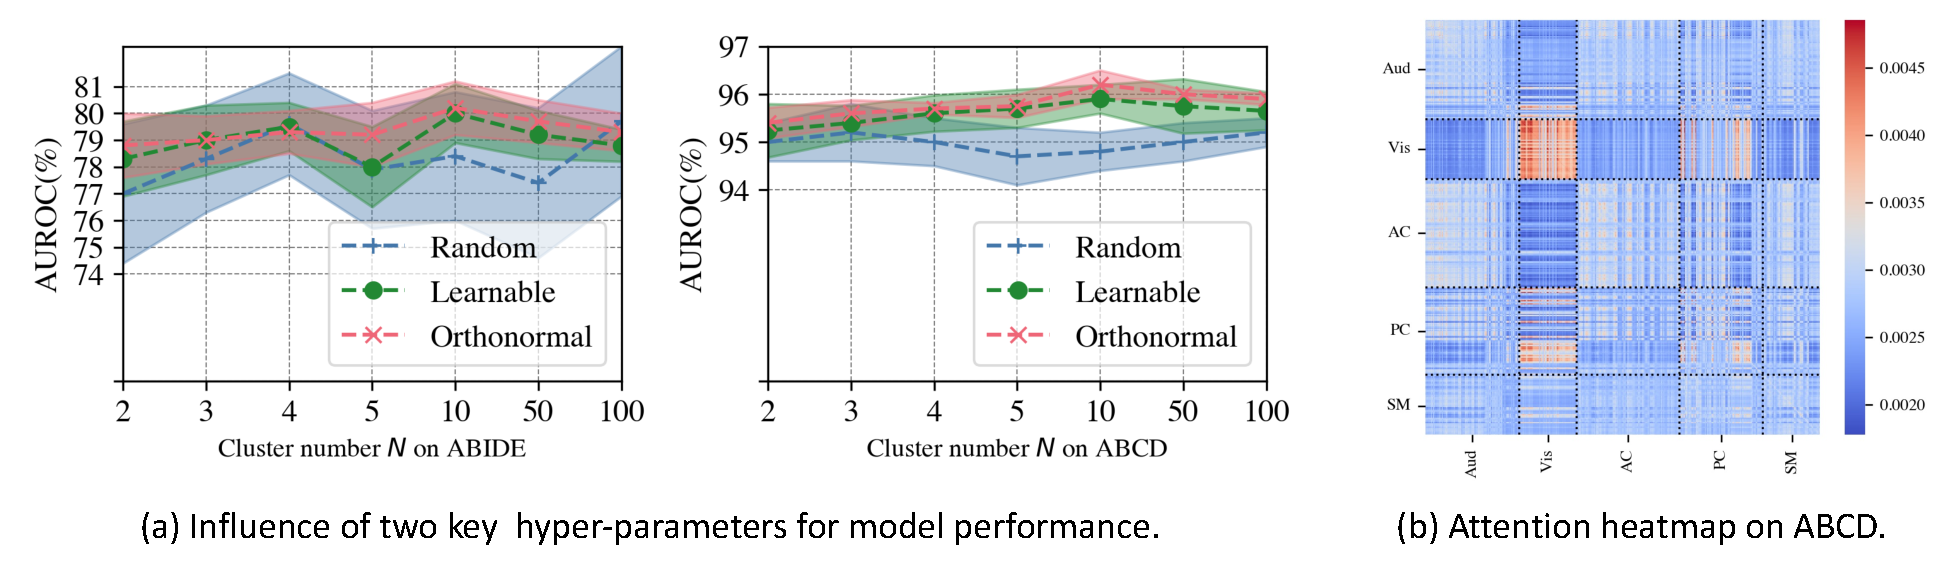
\includegraphics[width=0.90\linewidth]{figures/figure3.pdf}
    \caption{The hyper-parameter influence and the heatmap from self-attention.}
    \label{fig:parameter}
\end{figure*}

\subsection{In-depth Analysis of Attention Scores and Cluster Assignments (RQ3)}
Figure \ref{fig:parameter}(b) displays the self-attention score from the first layer of Multi-Head Self-Attention. The attention scores are the average across all subjects in the ABCD test set. This figure shows that the learned attention scores well match the divisions of functional modules based on available labels, demonstrating the effectiveness and explainability of our Transformer model. Note that since there exists no available functional module labels for the atlas of the ABIDE dataset, we cannot visualize the correlations between attention scores and functional modules.

Figure \ref{fig:soft_att} shows the cluster soft assignment results $\bm P$ on nodes in \poolingshort with two initialization methods. The cluster number $K$ is set to 4. The visualized numerical values are the average $\bm P$ of all subjects in each dataset's test set. From the visualization, we observe that (a) Base on Appendix~\ref{app:difference}, orthonormal initialization produces more discriminative $\bm P$ between classes than random initialization; (b) Within each class, orthonormal initialization encourages the nodes to form groups. These observations demonstrate that our \poolingshort with orthonormal initialization can leverage potential clusters underlying node embeddings, thus automatically grouping brain regions into potential functional modules. 

\begin{figure*}[h]
    \centering
    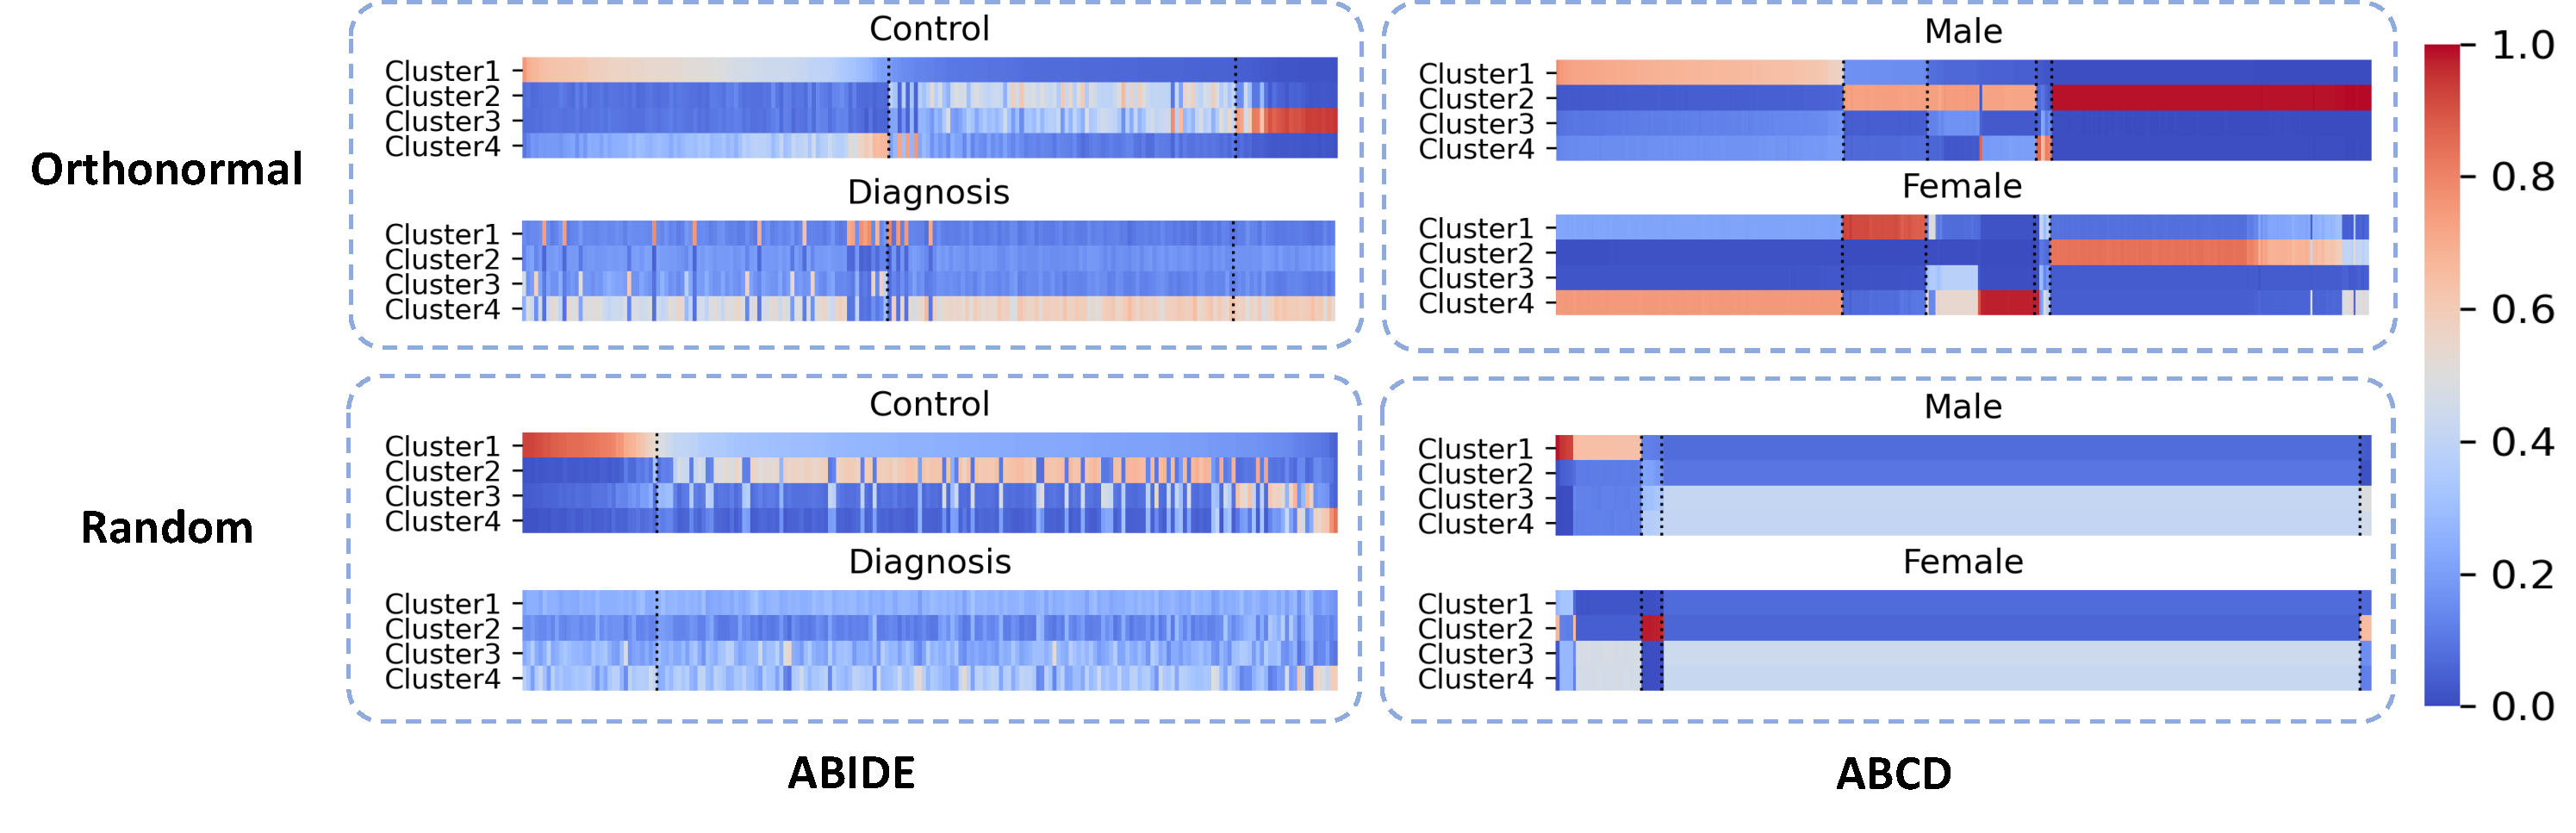
\includegraphics[width=0.9\linewidth]{figures/soft2.pdf}
    \caption{Visualization of cluster (module-level) embeddings learned with Orthonormal vs.~Random cluster center initializations on two datasets.  Each group in the dotted box contains two heatmaps (one for each prediction class) with the same node ordering on the x-axis.}
    \label{fig:soft_att}
\end{figure*}
 
	% ======================================================================================== %
\section{Conclusion}\label{sec:conclusion}
% ======================================================================================== %

In this paper, we proposed a variant of self-attention (SA), named phonetic self-attention (phSA), to improve the ASR performance.
Especially, we investigated the phonetic behavior of attention heads and distinguished two different attention patterns, similarity-based and content-based attention.
The proposed phSA emphasized the two behaviors by applying simple and effective modifications to the original dot-product in SA.
In addition, the effect of each behavior is controlled by additional trainable parameters.
From the phoneme classification experiments, we showed that phSA is more suitable than the vanilla SA for phonetic feature extraction.
By replacing SA in lower layers with phSA, we improved the speech recognition performance on the end-to-end Transformer-based ASR model.

	\section{Acknowledgments}

This research was supported in part by the University Research Committee of Emory University, and the internal funding and GPU servers provided by the Computer Science Department of Emory University. The authors gratefully acknowledge support from NIH under award number R01MH105561 and R01MH118771. The content is solely the responsibility of the authors and does not necessarily represent the official views of the National Institutes of Health. 

Data used in the preparation of this article were obtained from the Adolescent Brain Cognitive Development (ABCD) Study (\url{https://abcdstudy.org}), held in the NIMH Data Archive (NDA). This is a multisite, longitudinal study designed to recruit more than 10,000 children age 9-10 and follow them over 10 years into early adulthood. The ABCD Study\textsuperscript{\textregistered} is supported by the National Institutes of Health and additional federal partners under award numbers U01DA041048, U01DA050989, U01DA051016, U01DA041022, U01DA051018, U01DA051037, U01DA050987, U01DA041174, U01DA041106, U01DA041117, U01DA041028, U01DA041134, U01DA050988, U01DA051039, U01DA041156, U01DA041025, U01DA041120, U01DA051038, U01DA041148, U01DA041093, U01DA041089, U24DA041123, U24DA041147. A full list of supporters is available at  \sloppy\url{https://abcdstudy.org/federal-partners.html}. A listing of participating sites and a complete listing of the study investigators can be found at  \url{https://abcdstudy.org/consortium_members/}. ABCD consortium investigators designed and implemented the study and/or provided data but did not necessarily participate in the analysis or writing of this report. This manuscript reflects the views of the authors and may not reflect the opinions or views of the NIH or ABCD consortium investigators. The ABCD data repository grows and changes over time. The ABCD data used in this report came from NIMH Data Archive Release 4.0 (DOI 10.15154/1523041). DOIs can be found at \url{https://nda.nih.gov/abcd}.
\newpage
	
	\bibliographystyle{plain}
	\bibliography{reference}
	\clearpage
	\section*{Checklist}

\begin{enumerate}


\item For all authors...
\begin{enumerate}
  \item Do the main claims made in the abstract and introduction accurately reflect the paper's contributions and scope?
    \answerYes{}
  \item Did you describe the limitations of your work?
    \answerYes{} See Section \ref{sec:conclusion}.
  \item Did you discuss any potential negative societal impacts of your work?
    \answerNA{}
  \item Have you read the ethics review guidelines and ensured that your paper conforms to them?
    \answerYes{}
\end{enumerate}


\item If you are including theoretical results...
\begin{enumerate}
  \item Did you state the full set of assumptions of all theoretical results?
    \answerYes{} See Appendix \ref{app:prove}.
        \item Did you include complete proofs of all theoretical results?
    \answerYes{} See Appendix \ref{app:prove}.
\end{enumerate}


\item If you ran experiments...
\begin{enumerate}
  \item Did you include the code, data, and instructions needed to reproduce the main experimental results (either in the supplemental material or as a URL)?
    \answerYes{}
  \item Did you specify all the training details (e.g., data splits, hyperparameters, how they were chosen)?
    \answerYes{} See Implementation details in Section \ref{sec:expset}.
        \item Did you report error bars (e.g., with respect to the random seed after running experiments multiple times)?
    \answerYes{} See Metrics in Section \ref{sec:expset}.
        \item Did you include the total amount of compute and the type of resources used (e.g., type of GPUs, internal cluster, or cloud provider)?
    \answerYes{} See Implementation details in Section \ref{sec:expset}.
\end{enumerate}


\item If you are using existing assets (e.g., code, data, models) or curating/releasing new assets...
\begin{enumerate}
  \item If your work uses existing assets, did you cite the creators?
    \answerYes{} See Datasets in Section \ref{sec:expset}.
  \item Did you mention the license of the assets?
    \answerNA{} ABIDE and ABCD do not provide any license.
  \item Did you include any new assets either in the supplemental material or as a URL?
    \answerYes{} We provide our implementation and share our repository with MIT license.
  \item Did you discuss whether and how consent was obtained from people whose data you're using/curating?
    \answerYes{} See Datasets in Section \ref{sec:expset}.
  \item Did you discuss whether the data you are using/curating contains personally identifiable information or offensive content?
    \answerYes{} See Datasets in Section \ref{sec:expset}.
\end{enumerate}


\item If you used crowdsourcing or conducted research with human subjects...
\begin{enumerate}
  \item Did you include the full text of instructions given to participants and screenshots, if applicable?
    \answerNA{}
  \item Did you describe any potential participant risks, with links to Institutional Review Board (IRB) approvals, if applicable?
    \answerNA{}
  \item Did you include the estimated hourly wage paid to participants and the total amount spent on participant compensation?
    \answerNA{}
\end{enumerate}


\end{enumerate}
	\clearpage
	\appendix
	
\begin{table*}[t]
  \centering
  \begin{tabular}{llllllll}
  \toprule
  \multirow{2}{*}{\textbf{Persona}} & \multirow{2}{*}{\textbf{Method}} & \multicolumn{3}{c}{\textbf{Original}} & \multicolumn{3}{c}{\textbf{Revised}}\\
  & & \textbf{ppl} & \textbf{hits@1} & \textbf{F1}&\textbf{ppl} & \textbf{hits@1} & \textbf{F1}\\
  \midrule
  No Persona & & 38.08 & 0.092 & 0.168&38.08 & 0.092&0.168\\\midrule
  \multirow{3}{*}{Self Persona} & Seq2Seq & 40.53 & 0.084 &\textbf{0.172}& 40.65  & 0.082&\textbf{0.171}\\
   & Profile Memory & \textbf{34.54} & \textbf{0.125} &\textbf{0.172}& 38.21 & \textbf{0.108}&0.170\\\midrule
  \multirow{3}{*}{Their Persona} & Seq2Seq & 41.48 & 0.075 &0.168& 41.95 & 0.074&0.168\\
   & Profile Memory & 36.42 & 0.105 &0.167& \textbf{37.75} & 0.103&0.167\\\midrule
  \multirow{3}{*}{Both Personas} & Seq2Seq & 40.14 & 0.084 &0.169& 40.53 & 0.082&0.166\\
   & Profile Memory & 35.27 & 0.115 &0.171& 38.48 & 0.106&0.168\\ 
  \bottomrule
  \end{tabular}
  \caption{{\bf Evaluation of dialog utterance prediction with generative models} in four settings: conditioned on the speakers persona (``self persona''), the dialogue partner's persona (``their persona''), both or none. The personas are either the original source given to Turkers to condition the dialogue, or the revised personas that do not have word overlap. In the ``no persona'' setting, the models are equivalent, so we only report once.
     \label{tab:generative-results}
     }
\end{table*}



\begin{table*}[t]
  \begin{center}
  %   \resizebox{1\linewidth}{!}{
      % {
      \begin{tabular}{l|cc|cc|cc|cc }
      \toprule
      ~&  \multicolumn{2}{c}{No Persona} & \multicolumn{2}{|c}{Self Persona} & \multicolumn{2}{|c}{Their Persona} & \multicolumn{2}{|c}{Both Personas} \\ 
      Method & Orig & Rewrite & Orig & Rewrite & Orig & Rewrite & Orig & Rewrite \\ 
      \midrule
      IR baseline  &0.214 & 0.214 & 0.410 & 0.207  &  0.181  & 0.181 & 0.382& 0.188 \\
      \multicolumn{8}{l}{{\em Training on original personas}}\\
      Starspace    & 0.318 & 0.318 &  0.481  & 0.295& 0.245 & 0.235 & 0.429 & 0.258\\
      Profile Memory        &  0.318 & 0.318 & 0.473 & 0.302 & 0.283 & 0.267 & 0.438 & 0.266\\    
      \multicolumn{8}{l}{{\em Training on revised personas}}\\
      Starspace    &  0.318 & 0.318 & 0.491 & 0.322 & 0.271 & 0.261 & 0.432 & 0.288\\
      Profile Memory        &  0.318 & 0.318 & 0.509 & 0.354 & 0.299 & 0.294 & 0.467 & 0.331\\
      KV Profile Memory     &  0.349 & 0.349 & 0.511 & 0.351 & 0.291 &  0.289      &          0.467 &  0.330 \\
      \bottomrule
      \end{tabular}
      % }
      % }
      \caption{{\bf Evaluation of dialog utterance prediction with ranking models} using hits@1 in four settings: conditioned on the speakers persona ("self persona"), the dialogue partner's persona ("their persona"), both or none. The personas are either the original source given to Turkers to condition the dialogue, or the rewritten personas that do not have word overlap, explaining the poor performance of IR in that case. }
      \label{tab:retrieval-results}
  \end{center}
\end{table*}

\section{Next Utterance Prediction Additional Evaluation Metrics}

In Table \ref{tab:generative-results} and Table \ref{tab:retrieval-results} we show additional results on next utterance prediction.
In particular we give results for conditioning on the other person's persona ("Their") instead of one's own ("Self") or the combination ("Both"). In particular, we see that, knowing the other's persona does not help precision on this data with these models. Finally, we show in  Table \ref{tab:retrieval-results} for the ranking models the performance difference from training on original personas versus revised ones. Revised personas give improved results, perhaps because the models are forced to learn more than trivial word overlap (i.e. semantic similarity of differing phrases).


\section{Example Dialogs between Humans and Models}

In Tables \ref{table:os-example}, \ref{table:s2s-example}, \ref{table:kvp-example}, 
 \ref{table:opensubtitles2018-example}, \ref{table:twitter-example}
we show  example dialogues between Turkers
and various models that were collected as part of the human evaluation of Section \ref{sec:human-eval}.

\begin{table*}[t]
  \begin{center}
    \begin{small}
      \begin{tabular}{l|l}
        \toprule
        \textbf{Persona 1} & \textbf{Persona 2 (Not used by model)}\\
        \midrule
I am a doctor &  I eat sardines for breakfast daily \\
I have one brother & I just had surgery\\
My mom is a secretary & I love playing Frisbee \\
I like to eat a lot of meat & I have two large dogs \\
I am a bodybuilder & I never finished high school \\
\bottomrule
\multicolumn{2}{l}{ }\\
\multicolumn{2}{l}{[PERSON 1:] Hi I am Dr. Jenson. What is your name?}\\
\multicolumn{2}{l}{[PERSON 2:] Miss Dawes.}\\
\multicolumn{2}{l}{[PERSON 1:] Hi Miss Dawes, tell me about your family!}\\
\multicolumn{2}{l}{[PERSON 2:] Miss Baggoli, I know it must show on your records that my name is Mary, but everyone} \\\multicolumn{2}{l}{has referred to me as Lola since I was a squealing infant in my mother' s arms. }\\
\multicolumn{2}{l}{[PERSON 1:] fascinating. My secretary mother would have made note of all of that.}\\
\multicolumn{2}{l}{[PERSON 2:] In addition to the remainder, it writes my autobiography.}\\
\multicolumn{2}{l}{[PERSON 1:] Oh yeah? well I enjoy a nice steak. how about you?}\\
\multicolumn{2}{l}{[PERSON 2:] Father always used to say that if we ever had the money you have...}\\ \multicolumn{2}{l}{we' d have steak and ice cream three times every day!}\\
\multicolumn{2}{l}{[PERSON 1:] I eat all the steak and chicken too, even bacon}\\
\multicolumn{2}{l}{[PERSON 2:] Father always used to say that if we ever had the money you have...}\\ \multicolumn{2}{l}{we' d have steak and ice cream three times every day!}\\
\multicolumn{2}{l}{[PERSON 1:] yeah you said that already}\\
\multicolumn{2}{l}{[PERSON 2:] Dynamic structure can absorb shock.}\\
\multicolumn{2}{l}{[PERSON 1:] yes it can. I know about that as a bodybuilder}\\
\multicolumn{2}{l}{[PERSON 2:] Ladies and gentlemen... the strongest man in the world is blowing up a hot water bottle.}\\
      \end{tabular}
      \caption{Example dialog between a human (Person 1) and the OpenSubtitles KV Memory Network model (Person 2). %The Turker assigned a fluency score of 1 and engagingness of 1.
 \label{table:os-example}}
    \end{small}
  \end{center}
\end{table*}



\begin{table*}[t]
  \begin{center}
    \begin{small}
      \begin{tabular}{l|l}
        \toprule
        \textbf{Persona 1} & \textbf{Persona 2 (Not used by model)}\\
        \midrule
I am afraid of dogs & I am a carpenter \\
I used to work at a carnival & I used to drink but I stopped five years ago\\
I like to drink scotch to relax & I have a wife and three kids\\
I write short stories for a living & I like playing poker\\
I like dark superhero movies & I dont have many friends\\
\bottomrule
\multicolumn{2}{l}{ }\\
\multicolumn{2}{l}{[PERSON 1:] Hi are you relaxing on this fine evening?}\\
\multicolumn{2}{l}{[PERSON 2:] I am doing good and you?}\\
\multicolumn{2}{l}{[PERSON 1:] I am well, just drinking some scotch and working on my writing}\\
\multicolumn{2}{l}{[PERSON 2:] I love to cook and bake but I rarely make time for it} \\
\multicolumn{2}{l}{[PERSON 1:] what do you usually bake?}\\
\multicolumn{2}{l}{[PERSON 2:] I do not cook, I bake cakes at a local restaurant. how about you?}\\
\multicolumn{2}{l}{[PERSON 1:] I used to be a juggler at a carnival but now I am an author}\\
\multicolumn{2}{l}{[PERSON 2:] I am a dancer, what do you do?}\\ 
\multicolumn{2}{l}{[PERSON 1:] I just told you. Do you have any pets?}\\
\multicolumn{2}{l}{[PERSON 2:] no, I am allergic to pets unfortunately.}\\ 
\multicolumn{2}{l}{[PERSON 1:] I understand. I am not allergic but I am terrified of dogs!}\\
\multicolumn{2}{l}{[PERSON 2:] I have a cat. she has been with me through three wives, haha.}\\
\multicolumn{2}{l}{[PERSON 1:] Funny that you just told me you have no pets}\\
\multicolumn{2}{l}{[PERSON 2:] I do not have any animals.}\\
      \end{tabular}
      \caption{Example dialog between a human (Person 1) and the Seq2Seq model (Person 2). 
 \label{table:s2s-example}}
    \end{small}
  \end{center}
\end{table*}


\begin{table*}[t]
  \begin{center}
    \begin{small}
      \begin{tabular}{l|l}
        \toprule
        \textbf{Persona 1} & \textbf{Persona 2}\\
        \midrule
I am engaged to be married & I am a writer \\ 
I used to play sports in high school & I write romance novels\\
My favorite sport is soccer &  I live on a faraway island \\
I am a college graduate& I am an introvert \\
I love watching sports on TV& I have two cats \\
\bottomrule
\multicolumn{2}{l}{ }\\
\multicolumn{2}{l}{[PERSON 1:] I just got done playing soccer. What have you been up to?}\\
\multicolumn{2}{l}{[PERSON 2:] I do not have pets. I spend my free time writing. what about you?}\\
\multicolumn{2}{l}{[PERSON 1:] Just graduated from college. Looking for work. }\\
\multicolumn{2}{l}{[PERSON 2:] yes I graduated, in writing and poetry}\\
\multicolumn{2}{l}{[PERSON 1:] Have you had anything published?}\\
\multicolumn{2}{l}{[PERSON 2:] I mainly write fiction novels.}\\
\multicolumn{2}{l}{[PERSON 1:] Do you like to watch sports?}\\
\multicolumn{2}{l}{[PERSON 2:] do you like kings of leon my favorite by them is use somebody}\\
\multicolumn{2}{l}{[PERSON 1:] Are you married? I will be married soon. }\\
\multicolumn{2}{l}{[PERSON 2:] haha, no time. I have got a novel to finish.}\\
\multicolumn{2}{l}{[PERSON 1:] What is your novel about?}\\
\multicolumn{2}{l}{[PERSON 2:] it is a love story. I really enjoy writing. do you write or read?}\\
\multicolumn{2}{l}{[PERSON 1:] Like to read. Spend most time watching football. }\\
\multicolumn{2}{l}{[PERSON 2:] yes I do I am and author for a living}\\
      \end{tabular}
      \caption{Example dialog between a human (Person 1) and the Key-Value Profile Memory Network with Self Persona. %The Turker assigned a fluency score of 4, engagingness of 3, whilst correctly identifying the profile.
 \label{table:kvp-example}}
    \end{small}
  \end{center}
\end{table*}

\begin{table*}[t]
  \begin{center}
    \begin{small}
      \begin{tabular}{l|l}
        \toprule
        \textbf{Persona 1} & \textbf{Persona 2}\\
        \midrule
I dont like exercise or physical activity & My favorite type of food is Italian \\ 
My favorite food is ice cream & I have a big pet dog\\
I am a homebody &  I want to travel to Europe \\
 I have a husband who I love very much & I love reading books about travel \\
I love watching movies and TV& I like to walk long distances \\
\bottomrule
\multicolumn{2}{l}{ }\\
\multicolumn{2}{l}{[PERSON 1:] Hello, how are you doing today?}\\
\multicolumn{2}{l}{[PERSON 2:] I am good. I just got finished walking my dog.}\\
\multicolumn{2}{l}{[PERSON 1:] Oh cool! I am just sitting watching a movie. }\\
\multicolumn{2}{l}{[PERSON 2:] I have been watching that one before. I love it.}\\
\multicolumn{2}{l}{[PERSON 1:] Me too. I don't like going out much so I enjoy movies and TV.}\\
\multicolumn{2}{l}{[PERSON 2:] that is a great idea. I am going to read a book on writing.}\\
\multicolumn{2}{l}{[PERSON 1:] Oh, are you a writer?}\\
\multicolumn{2}{l}{[PERSON 2:] yes, I love to read. I am a great author.}\\
\multicolumn{2}{l}{[PERSON 1:] What sorts of topics do you write about?}\\
\multicolumn{2}{l}{[PERSON 2:] I could read all of those. I am sure you enjoy reading.}\\
\multicolumn{2}{l}{[PERSON 1:] I do, but I prefer movies.}\\
\multicolumn{2}{l}{[PERSON 2:] I have not, I can not do that. I have to go to the east coast.}\\
\multicolumn{2}{l}{[PERSON 1:] Why can't you watch movies?}\\
\multicolumn{2}{l}{[PERSON 2:] I have not. I have always had that done.}\\
      \end{tabular}
      \caption{Example dialog between a human (Person 1) and the Generative Profile Memory Network with Self Persona. %The Turker assigned a fluency score of 4, engagingness of 3, whilst correctly identifying the profile.
 \label{table:gpm-example}}
    \end{small}
  \end{center}
\end{table*}


\begin{table*}[t]
  \begin{center}
    \begin{small}
      \begin{tabular}{l|l}
        \toprule
        \textbf{Persona 1} & \textbf{Persona 2 (Not used by model)}\\
     \midrule   
I am very active & I am an engineering student \\ 
I live in the desert & I work at Eureka \\
I enjoy the outdoors & I like to celebrate with friends  \\
I was named something pretty common & I enjoy spending time with my toes in the sand\\
I instruct people how to get fit as a job &  I study to be a businessman \\
\bottomrule
\multicolumn{2}{l}{ }\\
\multicolumn{2}{l}{[PERSON 1:] Hello there, how are you?}\\
\multicolumn{2}{l}{[PERSON 2:] I'm fine.}\\
\multicolumn{2}{l}{[PERSON 1:] How is the weather, it is hot here }\\
\multicolumn{2}{l}{[PERSON 2:] It's so hot.}\\
\multicolumn{2}{l}{[PERSON 1:] oh yes tell me about it especially when you live in a desert.}\\
\multicolumn{2}{l}{[PERSON 2:] the sea is shining.}\\
\multicolumn{2}{l}{[PERSON 1:] you at the beach, i love the beach}\\
\multicolumn{2}{l}{[PERSON 2:] wait, wait, wait...}\\
\multicolumn{2}{l}{[PERSON 1:] what's up, you going somewhere }\\
\multicolumn{2}{l}{[PERSON 2:] you can be a good friend.}\\
\multicolumn{2}{l}{[PERSON 1:] yes, if you want me to}\\
\multicolumn{2}{l}{[PERSON 2:] I'm sorry.}\\
      \end{tabular}
      \caption{Example dialog between a human (Person 1) and the Language Model trained on the OpenSubtitles 2018 dataset (does not use persona). %The Turker assigned a fluency score of 4, engagingness of 3, whilst correctly identifying the profile.
 \label{table:opensubtitles2018-example}}
    \end{small}
  \end{center}
\end{table*}


\begin{table*}[t]
  \begin{center}
    \begin{small}
      \begin{tabular}{l|l}
        \toprule
        \textbf{Persona 1} & \textbf{Persona 2 (Not used by model)}\\
     \midrule   
I love ordering from Amazon & I really enjoy watching classic films over the new ones \\ 
I am a mother & My mother is the greatest chef in the world \\
I have a very active imagination & I stand out among my surroundings  \\
Winter holidays have always been my favorite & My son and daughter lived with me full time after I\\
I love the Harry Potter books &  \hspace{2em} separated from my husband\\
\bottomrule
\multicolumn{2}{l}{ }\\
\multicolumn{2}{l}{[PERSON 1:] Good afternoon! How are you?}\\
\multicolumn{2}{l}{[PERSON 2:] i'm not sure. I was just talking about the other day.}\\
\multicolumn{2}{l}{[PERSON 1:] Do you like to read? I like reading Harry Potter. }\\
\multicolumn{2}{l}{[PERSON 2:] I love you so much}\\
\multicolumn{2}{l}{[PERSON 1:] That's funny. You don't know me.}\\
\multicolumn{2}{l}{[PERSON 2:] I think you have to be a good person.}\\
\multicolumn{2}{l}{[PERSON 1:] Where do you live? Are you in the US?}\\
\multicolumn{2}{l}{[PERSON 2:] yes, I just found out that there were only 10 people who were in the city.}\\
\multicolumn{2}{l}{[PERSON 1:] Do you have any children? I am a mother to 1 cat. }\\
\multicolumn{2}{l}{[PERSON 2:] this is the first time in history, but not a few.}\\
\multicolumn{2}{l}{[PERSON 1:] Is it cold where you are?}\\
\multicolumn{2}{l}{[PERSON 2:] I don't even know what I'm talking about.}\\
      \end{tabular}
      \caption{Example dialog between a human (Person 1) and the Language Model trained on the Twitter dataset (does not use persona). %The Turker assigned a fluency score of 4, engagingness of 3, whilst correctly identifying the profile.
 \label{table:twitter-example}}
    \end{small}
  \end{center}
\end{table*}


\section{Human Evaluation Measures}

After dialogues between humans and a model, we then ask the Turker some additional questions in order to evaluate the quality of the model. 
They are, in order:
\begin{itemize}
\item {\bf Fluency}: We ask them to judge the fluency of the other speaker as a score from 1 to 5, where 1 is ``not fluent at all'', 5 is ``extremely fluent'', and 3 is ``OK''. 

\item {\bf Engagingness}: We ask them to judge the engagingness of the other speaker {\em disregarding fluency} from 1-5, where 1 is ``not engaging at all'', 5 is ``extremely engaging'', and 3 is ``OK''.

\item {\bf Consistency}: We ask them to judge the consistency of the persona of the other speaker, where we give the example that ``I have a dog''  followed by ``I have no pets'' is not consistent. The score is again from 1-5.

\item {\bf Profile Detection}: Finally, we display two possible profiles, and ask which is more likely to be the profile of the person the Turker just spoke to. One profile is chosen at random, and the other is the true persona given to the model.
\end{itemize}

\section{Profile Prediction}\label{app:profile-pred}

While the main study of this work is the ability to improve next utterance classification
by conditioning on a persona, 
one could naturally consider two tasks:
% studying dialogue conditioned on personas seems to 
%to naturally lead to two tasks:
(1) next utterance prediction during dialogue, and (2) profile prediction given dialogue history. 
In the main paper we show that Task 1 can be improved by using profile information.
Task 2, however, can be used to extract such information.

In this section we conduct a preliminary study of the ability to predict the persona
of a speaker given a set of dialogue utterances. 
We consider the dialogues between humans (PERSON 0)  and our best performing model, the retrieval-based Key-Value Profile Memory Network (PERSON 1) from Section \ref{sec:human-eval}. %\ref{sec:kvmem}) 
We tested the ability to predict the profile information of the two speakers from the dialogue
utterances of each speaker, considering all four combinations.
We employ the same 
IR baseline model used in the main paper to predict profiles: it ranks profile candidates, either at the entire profile level (considering all the sentences that make up the profile as a bag) or at the  sentence level (each  sentence individually). 
We consider 100 negative profile candidates for each positive profile, and compute the error rate of
predicting the true profile averaged over all dialogues and candidates.
The results are given in Table \ref{tab:task2a},  both for the model conditioned on profile information, and the same KV Memory model that is not.
The results indicate the following:
\begin{itemize}
\item It is possible to predict the humans profile from their dialogue utterances
(PERSON 0, Profile 0) with high accuracy at both the profile and sentence level, independent of the model they speaking to.
\item Similarly the model's profile can be predicted with high accuracy from its utterances (PERSON 1, Profile 1) when it is conditioned on the profile, otherwise this is chance level (w/o Profile).
\item It is possible to predict the model's profile from the human's dialogue, but with a lower accuracy (PERSON 0, Profile 1) as long as the model is conditioned on its own profile. This indicates the human responds to the model's utterances and pays attention to the model's interests. 
\item Similarly, the human's profile can be predicted from the model's dialogue, but with lower accuracy. Interestingly, the model without profile conditioning is better at this, perhaps because it does not concentrate on talking about itself, and pays more attention to responding to the human's interests. There appears to be a tradeoff that needs to be explored and understood here.
\end{itemize}

We also study the performance of profile prediction as the dialogue progresses, by computing error
rates for dialogue lengths 1 to 8 (the longest length we consider in this work). 
The results, given in Table \ref{tab:task2b}, show the error rate of predicting the persona 
decreases in all cases as dialogue length increases.

Overall, the results in this section 
show that it is plausible to predict profiles given dialogue utterances, which is
an important extraction task. Note that better results could likely be achieved with more sophisticated models.




\begin{table*}[t]
  \centering
  \begin{tabular}{ll|ll|ll}
  \toprule
  \multirow{3}{*}{\textbf{Speaker}} & 
  \multirow{3}{*}{\textbf{Profile}} & 
   \multicolumn{2}{c}{\textbf{Profile Level}} &   \multicolumn{2}{c}{\textbf{Sentence Level}} \\
%   &  \multicolumn{2}{l}{\textbf{KV Memory Network}} &  \multicolumn{2}{l}{\textbf{KV Memory Network}} \\
&   &  KV Profile & KV w/o Profile    &  KV Profile & KV w/o  Profile \\
  \midrule
PERSON 0 & Profile 0  &  0.057  &  0.017  & 0.173 & 0.141 \\
PERSON 0 & Profile 1  &  0.234  &  0.491 & 0.431 & 0.518 \\
PERSON 1 & Profile 0  &  0.254  &  0.112  & 0.431 & 0.349 \\
PERSON 1 & Profile 1  &  0.011  &  0.512  & 0.246 & 0.530 \\
  \bottomrule
  \end{tabular}
  \caption{{\bf Profile Prediction.}
     \label{tab:task2a}
  Error rates are given for predicting either the persona of speaker 0 (Profile 0) or
of speaker 1 (Profile 1) given the dialogue utterances of speaker 0 (PERSON 0) or speaker
1 (PERSON 1). This is shown for dialogues between humans (PERSON 0) and either the 
KV Profile Memory model (``KV Profile'') which conditions on its own profile, or
the KV Memory model (``KV w/o Profile'') which does not.
  }
\end{table*}



\begin{table*}[t]
  \centering
  \begin{tabular}{ll|llllllll}
  \toprule
  \multirow{2}{*}{\textbf{Speaker}} & 
  \multirow{2}{*}{\textbf{Profile}} & 
  \multicolumn{8}{c}{\textbf{Dialogue Length}} 
  \\
   & & 1 & 2 & 3 & 4 & 5 & 6 & 7 & 8 \\
  \midrule
PERSON 0 & Profile 0  & 0.76 &  0.47 &  0.35 & 0.29 & 0.23 & 0.19 & 0.17  & 0.17 \\
PERSON 0 & Profile 1  & 0.51 &  0.39 &  0.32 & 0.29 & 0.27 & 0.27 &  0.25 & 0.25 \\  
PERSON 1 & Profile 0  & 0.57 &  0.52 &  0.48 & 0.46 & 0.45 & 0.43 &  0.43 & 0.43 \\
PERSON 1 & Profile 1  & 0.81 &  0.58 &  0.48 & 0.47 & 0.45 & 0.44 &  0.43 & 0.43 \\  
  \bottomrule
  \end{tabular}
  \caption{{\bf Profile Prediction By Dialog Length.}
  Error rates are given for predicting either the persona of speaker 0 (Profile 0) or
of speaker 1 (Profile 1) given the dialogue utterances of speaker 0 (PERSON 0) or speaker
1 (PERSON 1). This is shown for dialogues between humans (PERSON 0) and the 
KV Profile Memory model averaged over the first $N$ dialogue utterances from 100 conversations 
(where $N$ is the ``Dialogue Length''). The results show the  accuracy of predicting the persona 
improves in all cases as dialogue length increases.
     \label{tab:task2b}
  }
\end{table*}










	
	
	
	
	% Optionally include extra information (complete proofs, additional experiments and plots) in the appendix.
	% This section will often be part of the supplemental material.
	
	
\end{document}
